\chapter{Organometaalkatalyse: elementaire stappen en cycli}\label{ch:b2:catalytic-cycles}

Een paar milligram van een palladiumzout kan twee \omterm{def:b2:huckel:aromatic}{aromatische} ringen verbinden in een kolf
met kilo's reagentia: hetzelfde metaalatoom doet het werk duizenden
keren, en keert na elke doorgang terug naar zijn begintoestand. Hoe het dat doet,
vertelt een \omterm{def:b2:catalytic-cycles:cycle}{katalytische cyclus}, een gesloten reeks van een handvol elementaire stappen.
Er bestaan maar een paar soorten stappen, en elk verandert de oxidatietoestand, de
elektronentelling en het aantal liganden van het metaal op een vaste manier. Met de
elektronentelling van \cref{ch:b2:coordination-complexes} kan een cyclus gelezen,
gecontroleerd en soms voorspeld worden.

\begin{recall}
\Cref{ch:b2:coordination-complexes}: oxidatietoestand, $d^n$, \omterm{def:b2:coordination-complexes:electron-count}{valentie-elektronentelling},
\omterm{def:b2:coordination-complexes:electron-count}{18-elektronenregel}, \omterm{def:b2:coordination-complexes:hapticity}{hapticiteit}. \Cref{ch:b2:ligand-field}: $\pi$-acceptorliganden en
\omterm{def:b2:ligand-field:pi-ligands}{terugdonatie}. Het deel van jaar~1: katalysator, homogene katalyse, elementaire stap,
snelheidsbepalende stap, organometaalverbinding, oxidatiegetal.
\end{recall}

\begin{omfigure}
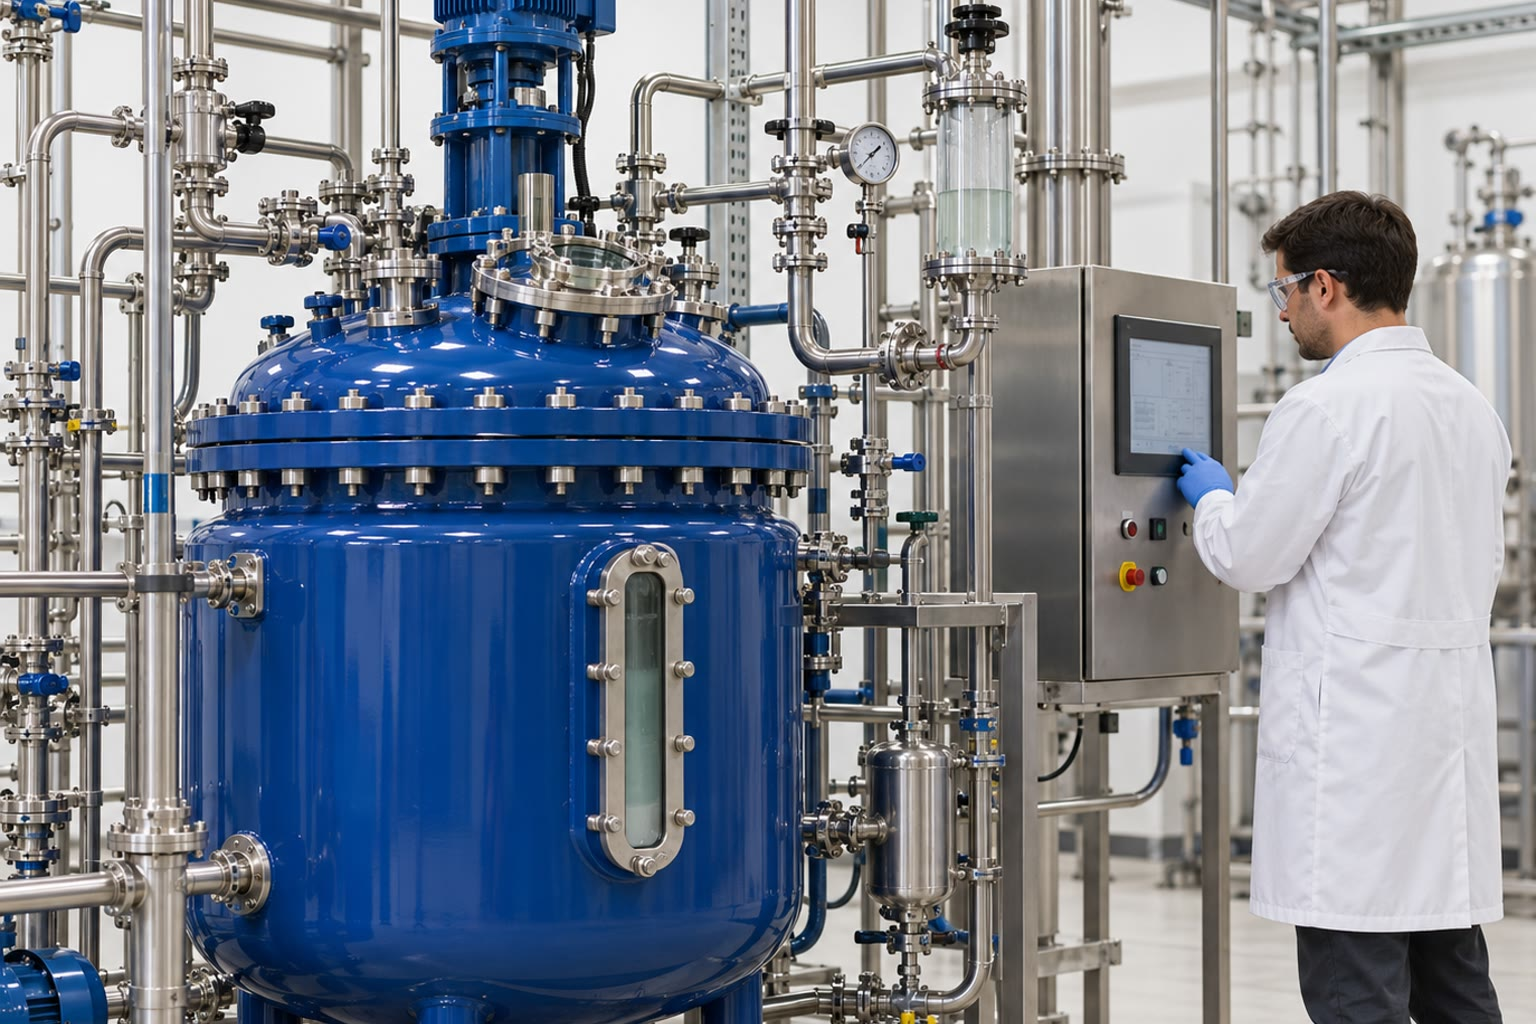
\includegraphics[width=0.62\linewidth]{images/book3/ai/b2-20-pilot-plant.jpg}

{\small Een proefinstallatie van de proceschemie: een geëmailleerde stalen reactor, waarin een
gekatalyseerde koppeling vanuit de kolf wordt opgeschaald vóór de productie.}
\end{omfigure}

\section{De taal van organometaalcomplexen}

Organometaalcomplexen worden geteld zoals in \cref{met:b2:coordination-complexes:electron-count},
met een paar extra liganden: een hydride \ce{H-} en een alkyl- of arylanion \ce{R-} leveren elk twee
elektronen en tellen $-1$ in de oxidatietoestand; \ce{CO}, fosfinen \ce{PR3} en
$\eta^2$-alkenen leveren twee elektronen en tellen 0; een halogenide \ce{X-} levert er twee en telt
$-1$.

\begin{definition}[Onverzadigde complexen]\label{def:b2:catalytic-cycles:unsaturated}
Een \emph{coördinatief onverzadigd complex}\index{coordinatief onverzadigd complex@coördinatief onverzadigd complex}
heeft minder dan 18 valentie-elektronen (vaak 16) en kan nog een ligand binden: het heeft een
\emph{vrije coördinatieplaats}\index{vrije coordinatieplaats@vrije coördinatieplaats}, een positie van zijn \omterm{def:b2:coordination-complexes:coordination-sphere}{coördinatiesfeer} die vrij is
om een donor van twee elektronen te ontvangen.
\end{definition}

Vlak vierkante $d^8$-complexen van rodium(I), iridium(I), palladium(II) en
platina(II) zijn complexen met 16 elektronen; palladium(0)-bisfosfinen \ce{PdL2} hebben er 14.
Zulke complexen zijn de actieve deeltjes van de meeste katalytische cycli.

\begin{method}[Een organometaalcomplex tellen]\label{met:b2:catalytic-cycles:count-organometallic}
\begin{enumerate}
  \item Som de liganden op: anionisch (\ce{H-}, \ce{R-}, \ce{X-}, \ce{C5H5-}) en neutraal
        (\ce{CO}, \ce{PR3}, alkenen, oplosmiddel).
  \item Oxidatietoestand = lading van het complex $-$ som van de ladingen van de anionische liganden.
  \item $n = g -$ oxidatietoestand; telling = $n + 2 \times$(aantal donoren van twee elektronen)
        $+$ 6 per $\eta^5$-\ce{C5H5-}.
  \item Coördinatiegetal = aantal bezette ligandposities.
\end{enumerate}
\end{method}

\section{Liganduitwisseling, oxidatieve additie, reductieve eliminatie}

\begin{definition}[Liganduitwisseling]\label{def:b2:catalytic-cycles:ligand-exchange}
Een \emph{liganduitwisseling}\index{liganduitwisseling} is een elementaire stap waarin een ligand van
de \omterm{def:b2:coordination-complexes:coordination-sphere}{coördinatiesfeer} door een ander vervangen wordt; ze verandert noch de oxidatietoestand,
noch, in totaal, de elektronentelling. Haar mechanismen worden bestudeerd in het deel van jaar~3.
\end{definition}

\begin{definition}[Oxidatieve additie en reductieve eliminatie]\label{def:b2:catalytic-cycles:oxidative-addition}
Bij een \emph{oxidatieve additie}\index{oxidatieve additie} addeert een molecuul A--B aan een
metaalcentrum door zijn binding A--B te verbreken en bindingen M--A en M--B te vormen. Een
\emph{reductieve eliminatie}\index{reductieve eliminatie} is de omgekeerde stap: twee
liganden A en B, cis ten opzichte van elkaar, verbinden zich tot A--B en verlaten het metaal.
\end{definition}

\begin{proposition}[Een oxidatieve additie tellen]\label{prop:b2:catalytic-cycles:oa}
Een \omterm{def:b2:catalytic-cycles:oxidative-addition}{oxidatieve additie} verhoogt de oxidatietoestand van het metaal met 2, zijn \omterm{def:b2:coordination-complexes:electron-count}{valentie-elektronentelling}
met 2 en zijn coördinatiegetal met 2; een \omterm{def:b2:catalytic-cycles:oxidative-addition}{reductieve eliminatie} verlaagt elk ervan met 2.
\end{proposition}

\begin{proof}
A en B worden, eenmaal gebonden, als anionen geteld (\ce{H-}, \ce{R-}, \ce{X-}): twee nieuwe anionische
liganden verhogen de oxidatietoestand met 2 en verlagen $n$ met 2; ze leveren twee paren, $+4$
elektronen; de telling verandert met $-2 + 4 = +2$. Twee posities worden nieuw bezet. De
omgekeerde stap keert elke verandering om.
\end{proof}

\begin{example}[Het complex van Vaska]\label{ex:b2:catalytic-cycles:vaska}
\ce{[IrCl(CO)(PPh3)2]}, vlak vierkant: iridium(I), $d^8$, 16 elektronen, coördinatiegetal vier.
Het addeert diwaterstof: \ce{[IrH2Cl(CO)(PPh3)2]}, iridium(III), $d^6$, 18 elektronen, octaëdrisch,
met de twee hydriden cis.
\end{example}

\section{Insertie, eliminatie, transmetallering}

\begin{definition}[Insertie en $\beta$-hydride-eliminatie]\label{def:b2:catalytic-cycles:insertion}
Bij een \emph{migratorische insertie}\index{migratorische insertie} voegt een onverzadigd ligand
(alkeen, \ce{CO}) dat aan het metaal gebonden is, zich in een cis staande binding M--H of M--C in: \ce{M-H} en een
alkeen geven een alkyl \ce{M-CH2-CH2-H}; \ce{M-R} en \ce{CO} geven een acyl \ce{M-C(=O)R}.
Een \emph{$\beta$-hydride-eliminatie}\index{beta-hydride-eliminatie@$\beta$-hydride-eliminatie}
is het omgekeerde van een alkeeninsertie: een waterstofatoom op het koolstofatoom in $\beta$ van het
metaal verhuist naar het metaal, waarbij een alkeen vrijkomt.
\end{definition}

\begin{proposition}[Een insertie tellen]\label{prop:b2:catalytic-cycles:insertion}
Een \omterm{def:b2:catalytic-cycles:insertion}{migratorische insertie} behoudt de oxidatietoestand en verlaagt de elektronentelling met 2
(er komt een ligandpositie vrij); een $\beta$-hydride-eliminatie verhoogt de telling met 2.
\end{proposition}

\begin{proof}
Ervoor: \ce{H-} (of \ce{R-}, anionisch) en het alkeen (neutraal), twee liganden, vier elektronen.
Erna: één alkyl (anionisch), twee elektronen. De anionische lading is onveranderd: dezelfde
oxidatietoestand; twee elektronen en één positie verloren.
\end{proof}

\begin{proposition}[Voorwaarden voor $\beta$-hydride-eliminatie]\label{prop:b2:catalytic-cycles:beta-h}
Een metaalalkyl ondergaat alleen $\beta$-hydride-eliminatie als de alkylgroep een waterstofatoom draagt op
haar $\beta$-koolstofatoom en het metaal een \omterm{def:b2:catalytic-cycles:unsaturated}{vrije coördinatieplaats} heeft die cis staat ten opzichte van de alkylgroep.
\end{proposition}

\begin{proof}[Redenering]
De stap verloopt via een vierledige schikking M--C$_\alpha$--C$_\beta$--H waarin het
waterstofatoom het metaal bereikt: ze vereist dat waterstofatoom, en een lege positie naast de alkylgroep
om het te ontvangen. Methyl-, benzyl-, neopentyl- en arylgroepen, die geen $\beta$-waterstof
hebben dat het metaal kan bereiken, zijn er stabiel tegen.
\end{proof}

\begin{definition}[Transmetallering]\label{def:b2:catalytic-cycles:transmetalation}
Een \emph{transmetallering}\index{transmetallering} brengt een organische groep over van het ene metaal
(of metalloïde: boor, zink, tin) naar een ander, meestal in ruil voor een halogenide.
\end{definition}

\begin{omfigure}
\begin{tikzpicture}[font=\small, >={Stealth}]
  \tikzset{omstepar/.style={->, thick}}
  \foreach \y/\l/\r/\top/\bot/\rev in {
      0/{$\mathrm{L}_n\mathrm{M}$}/{$\mathrm{L}_n\mathrm{M(A)(B)}$}/{+ A--B}/{oxidatieve additie}/{reductieve eliminatie},
      -1.5/{$\mathrm{L}_n\mathrm{M(H)(CH_2{=}CH_2)}$}/{$\mathrm{L}_n\mathrm{M{-}CH_2CH_3}$}/{}/{migratorische insertie}/{$\beta$-hydride-eliminatie},
      -3.0/{$\mathrm{L}_n\mathrm{M(X)(R)}$}/{$\mathrm{L}_n\mathrm{M(R)(R')}$}/{+ R$'$--[B], $-$ X--[B]}/{transmetallering}/{},
      -4.5/{$\mathrm{L}_n\mathrm{M(X)}$}/{$\mathrm{L}_n\mathrm{M(X)(L')}$}/{+ L$'$}/{liganduitwisseling of -binding}/{}} {
    \node[cyclenode, anchor=east] (l) at (0,\y) {\l};
    \node[cyclenode, anchor=west] (r) at (5.2,\y) {\r};
    \draw[omstepar] ($(l.east)+(0.1,0.08)$) -- ($(r.west)+(-0.1,0.08)$) node[midway, above, font=\scriptsize] {\top};
    \node[font=\scriptsize, anchor=north] at (2.6,\y-0.02) {\bot};
    \node[font=\scriptsize, black!55, anchor=west] at (5.2,\y-0.5) {\rev};
  }
\end{tikzpicture}

{\small De elementaire stappen van de organometaalkatalyse. \omterm{def:b2:catalytic-cycles:oxidative-addition}{Oxidatieve additie}: oxidatietoestand,
telling en coördinatiegetal $+2$; \omterm{def:b2:catalytic-cycles:oxidative-addition}{reductieve eliminatie}: $-2$. \omterm{def:b2:catalytic-cycles:insertion}{Migratorische
insertie}: telling $-2$, oxidatietoestand onveranderd; $\beta$-hydride-eliminatie: het
omgekeerde. \omterm{def:b2:catalytic-cycles:transmetalation}{Transmetallering}: een organische groep gaat van boor, zink of tin naar het metaal.}
\end{omfigure}

\section{Een katalytische cyclus lezen}

\begin{definition}[Katalytische cyclus]\label{def:b2:catalytic-cycles:cycle}
Een \emph{katalytische cyclus}\index{katalytische cyclus} is een gesloten reeks elementaire stappen
die de reagentia verbruikt, de producten vrijgeeft en zijn eerste complex regenereert. De
verbinding die aan de reactie wordt toegevoegd en die het eerste complex van de cyclus wordt, is de
\emph{prekatalysator}\index{prekatalysator}. Het \emph{turnovergetal}\index{turnovergetal}
(TON) is de hoeveelheid gevormd product per hoeveelheid katalysator; de
\emph{turnoverfrequentie}\index{turnoverfrequentie} (TOF) is het turnovergetal per tijdseenheid.
\end{definition}

\begin{proposition}[De totale vergelijking]\label{prop:b2:catalytic-cycles:cycle-sum}
De som van de stappen van een \omterm{def:b2:catalytic-cycles:cycle}{katalytische cyclus} is de vergelijking van de gekatalyseerde reactie:
elk metaalcomplex verschijnt één keer als product en één keer als beginstof, en valt weg.
\end{proposition}

\begin{proof}
Omdat de cyclus gesloten is, wordt elk intermediair gevormd door één stap en verbruikt door de volgende;
bij het optellen van de stappen verschijnen deze deeltjes aan beide kanten en vallen ze weg. Wat overblijft, zijn de
deeltjes die van buitenaf binnenkomen (reagentia) en vertrekken (producten).
\end{proof}

\begin{method}[Een cyclus lezen]\label{met:b2:catalytic-cycles:read-cycle}
\begin{enumerate}
  \item Bereken voor elk complex de oxidatietoestand, de elektronentelling en het
        coördinatiegetal.
  \item Benoem elke stap aan de hand van de veranderingen ($+2/+2/+2$: \omterm{def:b2:catalytic-cycles:oxidative-addition}{oxidatieve additie}; telling $-2$ bij
        constante oxidatietoestand: insertie; enzovoort).
  \item Controleer dat geen enkel complex meer dan 18 elektronen heeft en dat een stap die een \omterm{def:b2:catalytic-cycles:unsaturated}{vrije
        coördinatieplaats} nodig heeft, vertrekt van een onverzadigd complex.
  \item Tel de stappen op: de som moet de totale vergelijking zijn.
\end{enumerate}
\end{method}

\begin{omfigure}
\begin{tikzpicture}[font=\small, >={Stealth}]
  \node[cyclenode] (n1) at (90:2.3) {\ce{[RhCl(PPh3)2]}\\ Rh(I), 14 e};
  \node[cyclenode] (n2) at (0:3.4) {\ce{[RhH2Cl(PPh3)2]}\\ Rh(III), 16 e};
  \node[cyclenode] (n3) at (270:2.3) {\ce{[RhH2Cl(PPh3)2(RCH=CH2)]}\\ Rh(III), 18 e};
  \node[cyclenode] (n4) at (180:3.4) {\ce{[RhH(CH2CH2R)Cl(PPh3)2]}\\ Rh(III), 16 e};
  \draw[cyclearc] (n1) to[bend left=20] node[cyclelabel, below left] {oxidatieve\\ additie} (n2);
  \draw[cyclearc] (n2) to[bend left=20] node[cyclelabel, left=12pt] {binding\\ van het alkeen} (n3);
  \draw[cyclearc] (n3) to[bend left=20] node[cyclelabel, above right] {migratorische\\ insertie} (n4);
  \draw[cyclearc] (n4) to[bend left=20] node[cyclelabel, below right] {reductieve\\ eliminatie} (n1);
  \draw[cyclein] (4.6,2.3) node[right] {\ce{H2}} -- (2.6,1.75);
  \draw[cyclein] (4.6,-2.3) node[right] {alkeen} -- (2.6,-1.75);
  \draw[cycleout] (-2.6,1.75) -- (-4.6,2.3) node[left] {alkaan};
  \node[font=\scriptsize, align=center, black!60] at (0,-0.05) {prekatalysator\\ \ce{[RhCl(PPh3)3]}\\ verliest één \ce{PPh3}};
\end{tikzpicture}

{\small De hydrogenering van een alkeen met de katalysator van Wilkinson, vereenvoudigd (uitwisselingen van fosfine
en oplosmiddel weggelaten). De vier stappen tellen op tot $\ce{RCH=CH2 + H2 -> RCH2CH3}$; de
rodiumcomplexen vallen weg.}
\end{omfigure}

\begin{omfigure}
\begin{tikzpicture}[font=\small, >={Stealth}]
  \node[cyclenode] (s1) at (90:2.3) {\ce{PdL2}\\ Pd(0), 14 e};
  \node[cyclenode] (s2) at (0:3.4) {\ce{[ArPd(Br)L2]}\\ Pd(II), 16 e};
  \node[cyclenode] (s3) at (270:2.3) {$[\mathrm{ArPd(Ar')L_2}]$\\ Pd(II), 16 e};
  \draw[cyclearc] (s1) to[bend left=25] node[cyclelabel, below left] {oxidatieve\\ additie} (s2);
  \draw[cyclearc] (s2) to[bend left=25] node[cyclelabel, above left] {transmetallering} (s3);
  \draw[cyclearc] (s3) to[bend left=35] node[cyclelabel, right] {reductieve\\ eliminatie} (s1);
  \draw[cyclein] (4.8,2.2) node[right] {\ce{Ar-Br}} -- (2.6,1.6);
  \draw[cyclein] (5.4,-0.9) node[right, align=left] {$\mathrm{Ar'B(OH)_2}$\\ + base} -- (3.3,-1.2);
  \draw[cycleout] (2.3,-2.0) -- (4.4,-2.9) node[right] {\ce{Br-}, \ce{B(OH)3}};
  \draw[cycleout] (-1.75,-0.4) -- (-4.2,-0.4) node[left] {$\mathrm{Ar{-}Ar'}$};
\end{tikzpicture}

{\small De suzukikoppeling, vereenvoudigd. Palladium(0) addeert het arylbromide; de base
zet het boorzuur om in een boraat, dat zijn arylgroep overdraagt aan palladium; de twee
arylgroepen, in cispositie, worden geëlimineerd als het biaryl, waarbij palladium(0) geregenereerd wordt.}
\end{omfigure}

Bij de heckreactie bindt het arylpalladiumcomplex dat door \omterm{def:b2:catalytic-cycles:oxidative-addition}{oxidatieve additie} gevormd is, een
alkeen in plaats van een boraat; \omterm{def:b2:catalytic-cycles:insertion}{migratorische insertie} plaatst de arylgroep op het alkeen, en een
$\beta$-hydride-eliminatie geeft het gesubstitueerde alkeen vrij (meestal het trans-isomeer)
en een palladiumhydride, waaruit een base \ce{HBr} verwijdert om palladium(0) te regenereren.

Hydroformylering, de additie van \ce{H2} en \ce{CO} over een alkeen tot een aldehyde,
verloopt op hydriden van kobalt of rodium via insertie van het alkeen, insertie van \ce{CO}
in de binding metaal-alkyl, \omterm{def:b2:catalytic-cycles:oxidative-addition}{oxidatieve additie} van \ce{H2} en \omterm{def:b2:catalytic-cycles:oxidative-addition}{reductieve eliminatie} van het
aldehyde. De richting van de eerste insertie beslist over het product: het metaal op het
eindstandige koolstofatoom geeft het lineaire aldehyde, op het binnenste koolstofatoom het vertakte; omvangrijke
fosfinen begunstigen het lineaire product.

\begin{history}[Kruiskoppelingen]
\begin{minipage}[t]{0.36\linewidth}
\vspace{0pt}
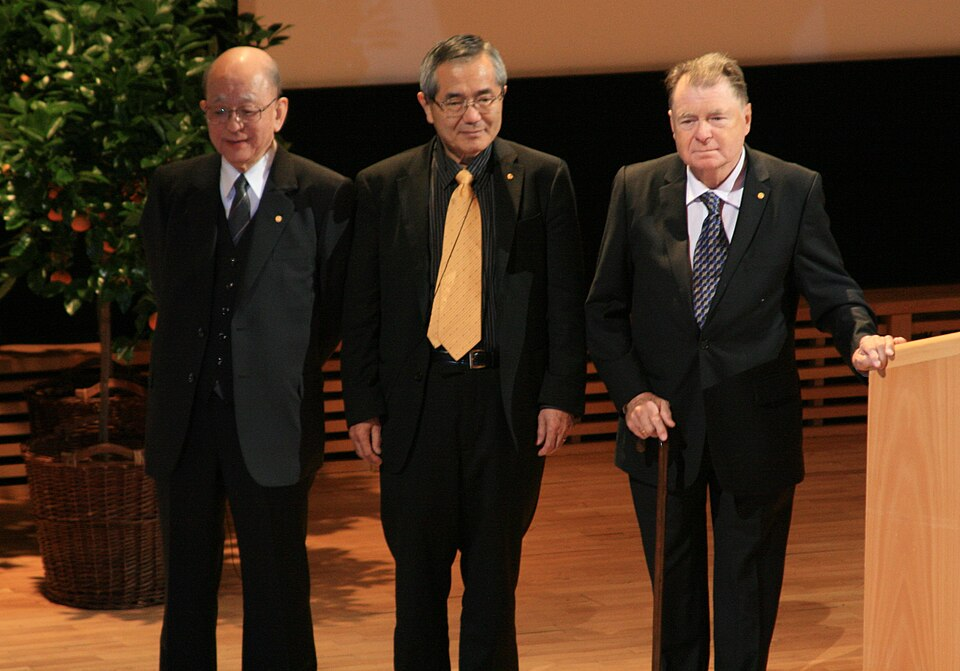
\includegraphics[width=\linewidth]{images/book3/nobel-2010.jpg}
\end{minipage}\hfill
\begin{minipage}[t]{0.6\linewidth}
\vspace{0pt}
Door palladium gekatalyseerde koppelingen van aryl- en vinylhalogeniden met alkenen (Richard Heck, vanaf
1968), met organozinkreagentia (Ei-ichi Negishi, 1977) en met organoboorverbindingen
(Akira Suzuki, 1979) maakten het verbinden van twee koolstofskeletten routine; ze behoren nu tot
de meest gebruikte reacties bij het maken van geneesmiddelen en materialen. De Nobelprijs voor
Scheikunde werd in 2010 aan de drie toegekend. (Foto: Suzuki, Negishi en Heck, van links
naar rechts, 2010; BloodIce, CC BY-SA 4.0, Wikimedia Commons.)
\end{minipage}
\end{history}

\begin{proposition}[Turnover]\label{prop:b2:catalytic-cycles:tof}
Met $n_P$ de hoeveelheid product die in een tijd $t$ door een hoeveelheid $n_{\text{kat}}$ katalysator gevormd wordt,
is $\mathrm{TON} = n_P/n_{\text{kat}}$ en is de gemiddelde \omterm{def:b2:catalytic-cycles:cycle}{turnoverfrequentie} $\mathrm{TOF} =
\mathrm{TON}/t$.
\end{proposition}

\begin{proof}
Elke omloop van de cyclus maakt één productmolecuul per metaalatoom; het aantal omlopen dat
elk atoom gemiddeld maakt, is $n_P/n_{\text{kat}}$, en de omloopsnelheid is dat aantal per
tijdseenheid.
\end{proof}

\begin{safety}{\ghs[5mm]{GHS05}\,\ghs[5mm]{GHS07}\,\ghs[5mm]{GHS09}}
Palladium(II)ethanoaat is corrosief voor de ogen en giftig voor waterorganismen;
trifenylfosfine is schadelijk en sensibiliserend. Ze worden in een zuurkast afgewogen, en de
palladiumresten worden ingezameld voor terugwinning, nooit door de gootsteen gespoeld.
% ledger: ghs:Pd-acetate, ghs:PPh3, ghs:phenylboronic-acid, ghs:4-bromotoluene
\end{safety}

\section{Oefeningen}

\begin{exercise}[$\star$]\label{exo:b2:catalytic-cycles:1}
Geef de oxidatietoestand, $d^n$ en de elektronentelling van het complex van Vaska
\ce{[IrCl(CO)(PPh3)2]} voor en nadat het \ce{H2} addeert.
\end{exercise}

\begin{exercise}[$\star$]\label{exo:b2:catalytic-cycles:2}
Benoem de stap: \ce{[PtCl2(CH3)2(PR3)2] -> [PtCl2(PR3)2] + C2H6}; \ce{[Pd(Ph)Br(PR3)2] +
CH2=CH2 -> [Pd(CH2CH2Ph)Br(PR3)] + PR3}.
\end{exercise}

\begin{exercise}[$\star$]\label{exo:b2:catalytic-cycles:3}
Een reactie gebruikt \qty{0.020}{mmol} katalysator en geeft \qty{15.0}{mmol} product in
\qty{3.0}{h}. Bereken het TON en de gemiddelde TOF.
\end{exercise}

\begin{exercise}[$\star$]\label{exo:b2:catalytic-cycles:4}
Tel de drie stappen van de suzukicyclus op en controleer dat palladium wegvalt.
\end{exercise}

\begin{exercise}[$\star\star$]\label{exo:b2:catalytic-cycles:5}
Welke van deze alkylpalladiumcomplexen kunnen $\beta$-hydride-eliminatie ondergaan:
\ce{Pd-CH3}, \ce{Pd-CH2CH3}, \ce{Pd-CH2C(CH3)3}, \ce{Pd-CH2Ph}, \ce{Pd-CH(CH3)2}?
\end{exercise}

\begin{exercise}[$\star\star$]\label{exo:b2:catalytic-cycles:6}
Voorspel het product van de heckreactie van joodbenzeen met methylpropenoaat, en de
geometrie ervan.
\end{exercise}

\begin{exercise}[$\star\star$]\label{exo:b2:catalytic-cycles:7}
Schrijf de lineaire en vertakte aldehyden op die ontstaan bij de hydroformylering van propeen, en
leg uit welke insertie tot elk ervan leidt.
\end{exercise}

\begin{exercise}[$\star\star$]\label{exo:b2:catalytic-cycles:8}
Waarom kan \ce{[RhCl(PPh3)3]} pas \ce{H2} adderen na het verlies van een fosfine, terwijl
\ce{[RhCl(PPh3)2]} het meteen addeert?
\end{exercise}

\begin{exercise}[$\star\star$]\label{exo:b2:catalytic-cycles:9}
Waarom is er bij de suzukikoppeling een base nodig, en wat doet die met het boorzuur?
\end{exercise}

\begin{exercise}[$\star\star\star$]\label{exo:b2:catalytic-cycles:10}
Een voorgestelde cyclus voor de hydrogenering van een alkeen op een $d^8$-complex \ce{ML3X} (16 e)
begint met het binden van het alkeen tot een complex met 20 elektronen, gevolgd door \omterm{def:b2:catalytic-cycles:oxidative-addition}{oxidatieve additie}
van \ce{H2}. Zoek de fout en verbeter de volgorde.
\end{exercise}

\begin{exercise}[$\star\star\star$]\label{exo:b2:catalytic-cycles:11}
De hoeveelheid product van een gekatalyseerde reactie groeit als $n_P(t) = n_{\max}(1 - \mathrm e^{-t/\tau})$
met $n_{\max} = \qty{10.0}{mmol}$, $\tau = \qty{40}{min}$ en \qty{0.010}{mmol} katalysator
(gegevens voor de oefening). Bereken de begin-TOF en het uiteindelijke TON.
\end{exercise}

\begin{exercise}[$\star\star\star$]\label{exo:b2:catalytic-cycles:12}
Stel een kruiskoppeling voor om 4-methoxybifenyl te bereiden, met een keuze van het halogenide en het
boorzuur, en schrijf de cyclus op.
\end{exercise}

\section{Probleem: de suzukicyclus lezen}

\begin{problem}[{Weekendprobleem --- de prekatalysator en het actieve palladium(0), de
oxidatieve additie, transmetallering en reductieve eliminatie van een suzukikoppeling, het
rendement en het turnovergetal, en de nevenreacties}]
\label{pb:b2:catalytic-cycles:1}
Proef (gegevens voor de oefening): \qty{10.0}{mmol} 4-broomtolueen, \qty{12.0}{mmol}
fenylboorzuur, \qty{20}{mmol} kaliumcarbonaat, \qty{0.050}{mmol} palladium(II)ethanoaat
en \qty{0.10}{mmol} trifenylfosfine in een mengsel van tolueen, ethanol en
water, verhit onder stikstof; geïsoleerd product: \qty{1.51}{g} 4-methylbifenyl. Molaire
massa's (\unit{g/mol}): 4-broomtolueen 171.04, fenylboorzuur 121.93, 4-methylbifenyl
168.24, palladium(II)ethanoaat 224.51.
% ledger: aw:C, aw:H, aw:Br, aw:B, aw:O, aw:Pd

\medskip
\noindent\textbf{Deel I --- De katalysator.}
\begin{enumerate}
  \item Geef de oxidatietoestand en $d^n$ van palladium in palladium(II)ethanoaat.
  \item In de kolf wordt het gereduceerd tot \ce{Pd(PPh3)2}. Geef zijn oxidatietoestand, $d^n$ en
        elektronentelling.
  \item Waarom is dat complex coördinatief onverzadigd?
  \item Waarom wordt de reactie onder stikstof uitgevoerd?
  \item Wat is de rol van de overmaat trifenylfosfine?
  \item Is palladium(II)ethanoaat de katalysator of de \omterm{def:b2:catalytic-cycles:cycle}{prekatalysator}?
\end{enumerate}

\medskip
\noindent\textbf{Deel II --- De stappen.}
\begin{enumerate}[resume]
  \item Schrijf de \omterm{def:b2:catalytic-cycles:oxidative-addition}{oxidatieve additie} van 4-broomtolueen op en tel het product.
  \item Wat doet het carbonaat met fenylboorzuur?
  \item Schrijf de \omterm{def:b2:catalytic-cycles:transmetalation}{transmetallering} op.
  \item Waarom moeten de twee arylgroepen vóór de volgende stap cis staan?
  \item Schrijf de \omterm{def:b2:catalytic-cycles:oxidative-addition}{reductieve eliminatie} op en tel het palladiumdeeltje dat ontstaat.
  \item Tel de drie stappen op.
\end{enumerate}

\medskip
\noindent\textbf{Deel III --- Rendement en turnover.}
\begin{enumerate}[resume]
  \item Welk reagens is beperkend?
  \item Bereken de geïsoleerde hoeveelheid product.
  \item Bereken het rendement.
  \item Bereken de katalysatorbelading in mol~\% ten opzichte van het bromide.
  \item Bereken het \omterm{def:b2:catalytic-cycles:cycle}{turnovergetal} van palladium.
  \item De proef duurde \qty{4.0}{h}. Bereken de gemiddelde \omterm{def:b2:catalytic-cycles:cycle}{turnoverfrequentie} per uur.
\end{enumerate}

\medskip
\noindent\textbf{Deel IV --- Nevenreacties.}
\begin{enumerate}[resume]
  \item Er wordt wat bifenyl \ce{Ph-Ph} gevonden. Opper hoe het ontstaat.
  \item Waarom is hier geen $\beta$-hydride-eliminatie mogelijk?
  \item Een arylchloride reageert veel trager dan het bromide. Welke stap lijdt daaronder?
  \item Wat gebeurt er met het palladium aan het einde van de reactie, en waarom wordt het teruggewonnen?
  \item Waarom wordt een kleine overmaat boorzuur gebruikt?
  \item Geef het \omterm{def:b2:catalytic-cycles:cycle}{turnovergetal} van palladium in de proef.
\end{enumerate}
\end{problem}
